\documentclass[manuscript, nonacm, dvipsnames]{acmart}
\settopmatter{printacmref=false, printfolios=true}
\renewcommand\footnotetextcopyrightpermission[1]{}
\usepackage{booktabs}
\usepackage{standalone}
\usepackage{placeins}
\usepackage{float}
% analysis/style.tex — shared pgfplots preamble; % analysis/style.tex — shared pgfplots preamble; % analysis/style.tex — shared pgfplots preamble; \input{../style} from figures/
\usepackage[eulergreek]{sansmath}
\usepackage{pgfplots}
\usepackage{pgfplotstable}
\usepackage{xspace}

% Scheme-name macros — mirror the paper's meta/templates.tex so figure
% legends/titles/captions can write \plaintext / \sap / \emvp / \bntm /
% \tiptoe and render identically in both contexts. `\providecommand`
% lets the paper's templates.tex (loaded earlier) win when this file
% is in the paper as plots/pgfstyle.tex; in standalone artefact compiles
% these are the source of the macros.
\providecommand{\plaintext}{\textsc{Plaintext}\xspace}
\providecommand{\sap}{\textsc{SAP}\xspace}
\providecommand{\emvp}{\textsc{EMVP}\xspace}
\providecommand{\bntm}{\textsc{BNTM}\xspace}
\providecommand{\tiptoe}{\textsc{Tiptoe}\xspace}

\pgfplotsset{compat=newest}
\usepgfplotslibrary{units,colorbrewer,groupplots,fillbetween,statistics}
\usetikzlibrary{arrows.meta,backgrounds,calc,fit,shapes.geometric,positioning,patterns,shapes.misc}

% Bar charts request the colorbrewer Paired-12 cycle list directly via
% `cycle list/Paired-12` (loaded above by \usepgfplotslibrary{colorbrewer}).
% The library's `Paired-N` lists are full-colour, paper-quality, and live
% inside pgfplots so we don't ship a hand-rolled equivalent here.

\pgfplotsset{
  width=3.25in, height=2.5in,
  every axis/.append style={
    semithick,
    ymajorgrids=true,
    label style={font=\sffamily\small},
    title style={font=\sffamily\small},
  },
  % Line plots default to thick. `smooth` is NOT global — it is
  % opt-in per figure (added inside the axis options of figures 01,
  % 02, 04, 05, 06 that benefit from cubic interpolation). Putting
  % `smooth` in the global default fights pgfplots' `ybar` state
  % machine in figure 03 and `[only marks]` plots elsewhere; the
  % per-figure opt-in is cleaner than chasing local overrides.
  every axis plot/.append style={thick},
  legend style={
    draw=none,
    % Fully transparent legend container so overlap with plot title /
    % data points is visually obvious during figure tuning, rather
    % than silently masked. `fill=none` alone leaves an opaque white
    % rectangle on some pgfplots versions; pinning `fill opacity=0`
    % belt-and-braces guarantees see-through.
    fill=none,
    text opacity=1,
    anchor=south,
    at={(0.5,1)},
    font=\sffamily\small,
  },
  legend cell align=left,
  legend columns=-1,
  xtick align=outside,
  xtick pos=bottom,
  major tick length=1mm,
  tick label style={font=\sansmath\sffamily\small},
  every axis label={font=\sffamily\small},
  label style={font=\sffamily\small},
  {cycle list/Dark2},
  {cycle list/Set1},
  cycle list name=Dark2,
  cycle multiindex* list={
    Dark2\nextlist
    {solid,dashed,dotted,dashdotted,densely dashdotdotted}\nextlist
    mark list*\nextlist
  },
  /pgfplots/short line legend/.style={
    legend image code/.code={
      \draw[mark repeat=2,mark phase=2,##1]
        plot coordinates {(0cm,0cm)(0.2cm,0cm)(0.4cm,0cm)};
    }
  },
  /pgfplots/ybar legend/.style={
    /pgfplots/legend image code/.code={
      \draw[##1,/tikz/.cd,yshift=-0.25em](0cm,0cm) rectangle (4pt,6pt);
    },
  },
  /pgfplots/xbar legend/.style={
    /pgfplots/legend image code/.code={
      \draw[##1,/tikz/.cd,yshift=-0.25em](0cm,0cm) rectangle (4pt,6pt);
    },
  },
  select coords between index/.style 2 args={
    x filter/.code={
      \ifnum\coordindex<#1\def\pgfmathresult{}\fi
      \ifnum\coordindex>#2\def\pgfmathresult{}\fi
    }
  },
  discard if not/.style 2 args={
    x filter/.code={
      \edef\tempa{\thisrow{#1}}
      \edef\tempb{#2}
      \ifx\tempa\tempb
      \else
        \def\pgfmathresult{inf}
      \fi
    }
  },
}
 from figures/
\usepackage[eulergreek]{sansmath}
\usepackage{pgfplots}
\usepackage{pgfplotstable}
\usepackage{xspace}

% Scheme-name macros — mirror the paper's meta/templates.tex so figure
% legends/titles/captions can write \plaintext / \sap / \emvp / \bntm /
% \tiptoe and render identically in both contexts. `\providecommand`
% lets the paper's templates.tex (loaded earlier) win when this file
% is in the paper as plots/pgfstyle.tex; in standalone artefact compiles
% these are the source of the macros.
\providecommand{\plaintext}{\textsc{Plaintext}\xspace}
\providecommand{\sap}{\textsc{SAP}\xspace}
\providecommand{\emvp}{\textsc{EMVP}\xspace}
\providecommand{\bntm}{\textsc{BNTM}\xspace}
\providecommand{\tiptoe}{\textsc{Tiptoe}\xspace}

\pgfplotsset{compat=newest}
\usepgfplotslibrary{units,colorbrewer,groupplots,fillbetween,statistics}
\usetikzlibrary{arrows.meta,backgrounds,calc,fit,shapes.geometric,positioning,patterns,shapes.misc}

% Bar charts request the colorbrewer Paired-12 cycle list directly via
% `cycle list/Paired-12` (loaded above by \usepgfplotslibrary{colorbrewer}).
% The library's `Paired-N` lists are full-colour, paper-quality, and live
% inside pgfplots so we don't ship a hand-rolled equivalent here.

\pgfplotsset{
  width=3.25in, height=2.5in,
  every axis/.append style={
    semithick,
    ymajorgrids=true,
    label style={font=\sffamily\small},
    title style={font=\sffamily\small},
  },
  % Line plots default to thick. `smooth` is NOT global — it is
  % opt-in per figure (added inside the axis options of figures 01,
  % 02, 04, 05, 06 that benefit from cubic interpolation). Putting
  % `smooth` in the global default fights pgfplots' `ybar` state
  % machine in figure 03 and `[only marks]` plots elsewhere; the
  % per-figure opt-in is cleaner than chasing local overrides.
  every axis plot/.append style={thick},
  legend style={
    draw=none,
    % Fully transparent legend container so overlap with plot title /
    % data points is visually obvious during figure tuning, rather
    % than silently masked. `fill=none` alone leaves an opaque white
    % rectangle on some pgfplots versions; pinning `fill opacity=0`
    % belt-and-braces guarantees see-through.
    fill=none,
    text opacity=1,
    anchor=south,
    at={(0.5,1)},
    font=\sffamily\small,
  },
  legend cell align=left,
  legend columns=-1,
  xtick align=outside,
  xtick pos=bottom,
  major tick length=1mm,
  tick label style={font=\sansmath\sffamily\small},
  every axis label={font=\sffamily\small},
  label style={font=\sffamily\small},
  {cycle list/Dark2},
  {cycle list/Set1},
  cycle list name=Dark2,
  cycle multiindex* list={
    Dark2\nextlist
    {solid,dashed,dotted,dashdotted,densely dashdotdotted}\nextlist
    mark list*\nextlist
  },
  /pgfplots/short line legend/.style={
    legend image code/.code={
      \draw[mark repeat=2,mark phase=2,##1]
        plot coordinates {(0cm,0cm)(0.2cm,0cm)(0.4cm,0cm)};
    }
  },
  /pgfplots/ybar legend/.style={
    /pgfplots/legend image code/.code={
      \draw[##1,/tikz/.cd,yshift=-0.25em](0cm,0cm) rectangle (4pt,6pt);
    },
  },
  /pgfplots/xbar legend/.style={
    /pgfplots/legend image code/.code={
      \draw[##1,/tikz/.cd,yshift=-0.25em](0cm,0cm) rectangle (4pt,6pt);
    },
  },
  select coords between index/.style 2 args={
    x filter/.code={
      \ifnum\coordindex<#1\def\pgfmathresult{}\fi
      \ifnum\coordindex>#2\def\pgfmathresult{}\fi
    }
  },
  discard if not/.style 2 args={
    x filter/.code={
      \edef\tempa{\thisrow{#1}}
      \edef\tempb{#2}
      \ifx\tempa\tempb
      \else
        \def\pgfmathresult{inf}
      \fi
    }
  },
}
 from figures/
\usepackage[eulergreek]{sansmath}
\usepackage{pgfplots}
\usepackage{pgfplotstable}
\usepackage{xspace}

% Scheme-name macros — mirror the paper's meta/templates.tex so figure
% legends/titles/captions can write \plaintext / \sap / \emvp / \bntm /
% \tiptoe and render identically in both contexts. `\providecommand`
% lets the paper's templates.tex (loaded earlier) win when this file
% is in the paper as plots/pgfstyle.tex; in standalone artefact compiles
% these are the source of the macros.
\providecommand{\plaintext}{\textsc{Plaintext}\xspace}
\providecommand{\sap}{\textsc{SAP}\xspace}
\providecommand{\emvp}{\textsc{EMVP}\xspace}
\providecommand{\bntm}{\textsc{BNTM}\xspace}
\providecommand{\tiptoe}{\textsc{Tiptoe}\xspace}

\pgfplotsset{compat=newest}
\usepgfplotslibrary{units,colorbrewer,groupplots,fillbetween,statistics}
\usetikzlibrary{arrows.meta,backgrounds,calc,fit,shapes.geometric,positioning,patterns,shapes.misc}

% Bar charts request the colorbrewer Paired-12 cycle list directly via
% `cycle list/Paired-12` (loaded above by \usepgfplotslibrary{colorbrewer}).
% The library's `Paired-N` lists are full-colour, paper-quality, and live
% inside pgfplots so we don't ship a hand-rolled equivalent here.

\pgfplotsset{
  width=3.25in, height=2.5in,
  every axis/.append style={
    semithick,
    ymajorgrids=true,
    label style={font=\sffamily\small},
    title style={font=\sffamily\small},
  },
  % Line plots default to thick. `smooth` is NOT global — it is
  % opt-in per figure (added inside the axis options of figures 01,
  % 02, 04, 05, 06 that benefit from cubic interpolation). Putting
  % `smooth` in the global default fights pgfplots' `ybar` state
  % machine in figure 03 and `[only marks]` plots elsewhere; the
  % per-figure opt-in is cleaner than chasing local overrides.
  every axis plot/.append style={thick},
  legend style={
    draw=none,
    % Fully transparent legend container so overlap with plot title /
    % data points is visually obvious during figure tuning, rather
    % than silently masked. `fill=none` alone leaves an opaque white
    % rectangle on some pgfplots versions; pinning `fill opacity=0`
    % belt-and-braces guarantees see-through.
    fill=none,
    text opacity=1,
    anchor=south,
    at={(0.5,1)},
    font=\sffamily\small,
  },
  legend cell align=left,
  legend columns=-1,
  xtick align=outside,
  xtick pos=bottom,
  major tick length=1mm,
  tick label style={font=\sansmath\sffamily\small},
  every axis label={font=\sffamily\small},
  label style={font=\sffamily\small},
  {cycle list/Dark2},
  {cycle list/Set1},
  cycle list name=Dark2,
  cycle multiindex* list={
    Dark2\nextlist
    {solid,dashed,dotted,dashdotted,densely dashdotdotted}\nextlist
    mark list*\nextlist
  },
  /pgfplots/short line legend/.style={
    legend image code/.code={
      \draw[mark repeat=2,mark phase=2,##1]
        plot coordinates {(0cm,0cm)(0.2cm,0cm)(0.4cm,0cm)};
    }
  },
  /pgfplots/ybar legend/.style={
    /pgfplots/legend image code/.code={
      \draw[##1,/tikz/.cd,yshift=-0.25em](0cm,0cm) rectangle (4pt,6pt);
    },
  },
  /pgfplots/xbar legend/.style={
    /pgfplots/legend image code/.code={
      \draw[##1,/tikz/.cd,yshift=-0.25em](0cm,0cm) rectangle (4pt,6pt);
    },
  },
  select coords between index/.style 2 args={
    x filter/.code={
      \ifnum\coordindex<#1\def\pgfmathresult{}\fi
      \ifnum\coordindex>#2\def\pgfmathresult{}\fi
    }
  },
  discard if not/.style 2 args={
    x filter/.code={
      \edef\tempa{\thisrow{#1}}
      \edef\tempb{#2}
      \ifx\tempa\tempb
      \else
        \def\pgfmathresult{inf}
      \fi
    }
  },
}

\renewcommand{\sansmath}{}
\pgfplotsset{width=0.88\linewidth, height=0.44\linewidth}
\def\datadir{data}
\newcommand{\inputplot}[1]{\input{#1}}
\hypersetup{hidelinks}

\input{data/header}
% \canonicalSeries auto-generated by preprocess.py from the
% (machine, device, threads, cgroup) tuples that actually have data,
% rather than being hand-maintained. Adding a new machine to the
% fleet is a no-op now; just `make cross_machine` and the new series
% appear in every line plot via the figures' `\foreach` iteration.
\input{data/series}

\title{Cross-machine insights}
\subtitle{\insightsSubtitle}
\author{Secure Vector Search}
\affiliation{\institution{EPFL}\city{Lausanne}\country{Switzerland}}
\email{~}

\begin{document}
\maketitle

\section*{Machines}
\noindent\resizebox{\linewidth}{!}{%
\input{data/machines-table}}

\subsection*{Coverage}
\input{data/coverage-table}

\subsection*{Reading the figures}
Series legend labels encode (machine name, device, rayon-realised
thread count, cgroup CPU quota). The \texttt{GPU} suffix marks runs
that used a GPU per Plan~17's \texttt{device} axis. The
\texttt{t=N} suffix appears when the rayon pool size disagrees with
the host's logical core count --- typically a cgroup-shaped pod.
\texttt{cg=Q} reports the cgroup~v2 CPU quota in vCPU equivalents
(\texttt{/sys/fs/cgroup/cpu.max}); absence means no enforced cap on
that run.

\clearpage
\section{Latency vs nprobe (IVF schemes)}

\begin{figure}[H]
  \centering
  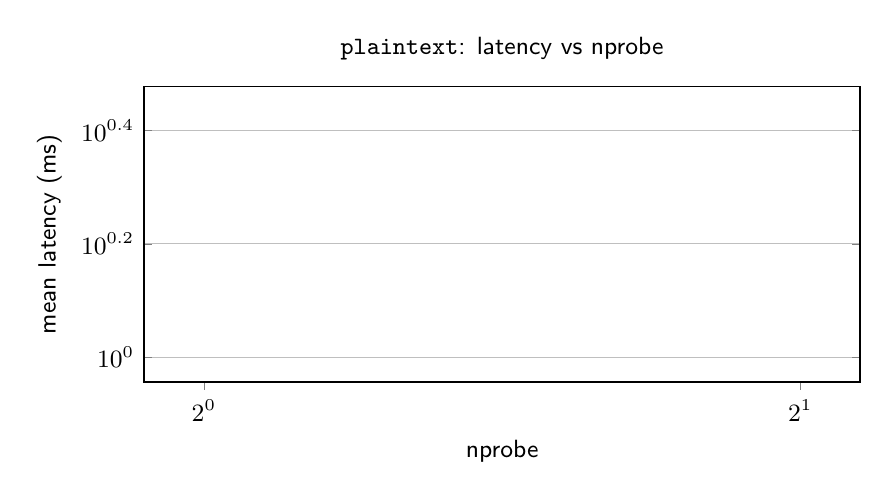
\begin{tikzpicture}
  \begin{axis}[
    xmode=log, log basis x=2, ymode=log,
    xlabel={nprobe},
    ylabel={mean latency (ms)},
    title={\texttt{plaintext}: latency vs nprobe},
    legend columns=3,
  ]
    % \foreach defines \slug and \dlabel only inside the loop body;
    % \addlegendentry stores its argument as a token list that pgfplots
    % renders after the axis ends, by which time \dlabel is gone. The
    % \edef + \noexpand dance below expands \slug and \dlabel right
    % now (per iteration) while leaving \addplot / \addlegendentry
    % themselves unevaluated.
    \foreach \slug/\dlabel in \canonicalSeries {%
      \IfFileExists{\datadir/01-latency-vs-nprobe-plaintext-\slug.tsv}{%
        \edef\xtemp{%
          \noexpand\addplot+ table[x=nprobe, y=latency_ms]
            {\datadir/01-latency-vs-nprobe-plaintext-\slug.tsv};%
          \noexpand\addlegendentry{\dlabel}%
        }\xtemp
      }{}%
    }
  \end{axis}
\end{tikzpicture}

  \caption{\texttt{plaintext} IVF: mean per-query latency vs
  \texttt{nprobe}, one series per (machine, device, threads, cgroup)
  tuple with recorded data. Higher \texttt{nprobe} trades latency for
  recall; the recall axis is suppressed here in favour of the
  hardware comparison.}
\end{figure}

\begin{figure}[H]
  \centering
  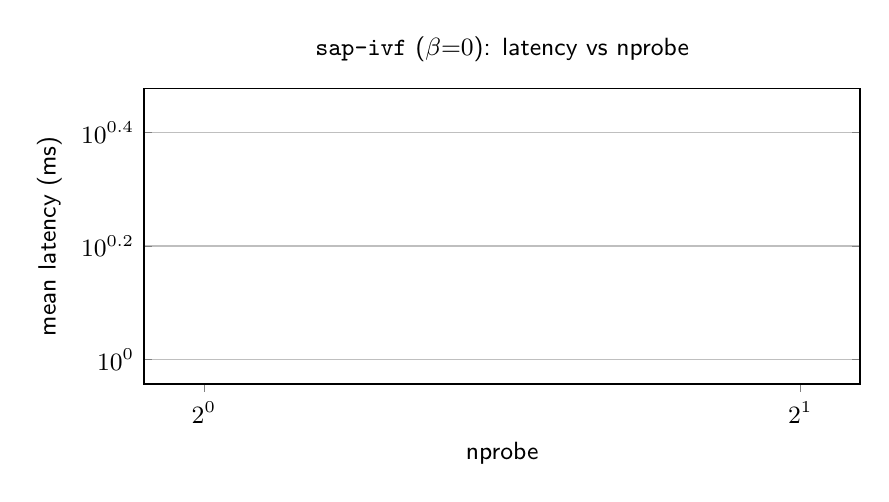
\begin{tikzpicture}
  \begin{axis}[
    xmode=log, log basis x=2, ymode=log,
    xlabel={nprobe},
    ylabel={mean latency (ms)},
    title={\texttt{sap-ivf} ($\beta{=}0$): latency vs nprobe},
    legend columns=3,
  ]
    \foreach \slug/\dlabel in \canonicalSeries {%
      \IfFileExists{\datadir/01-latency-vs-nprobe-sap-ivf-\slug.tsv}{%
        \edef\xtemp{%
          \noexpand\addplot+ table[x=nprobe, y=latency_ms]
            {\datadir/01-latency-vs-nprobe-sap-ivf-\slug.tsv};%
          \noexpand\addlegendentry{\dlabel}%
        }\xtemp
      }{}%
    }
  \end{axis}
\end{tikzpicture}

  \caption{\texttt{sap-ivf} at $\beta=0$: mean latency vs
  \texttt{nprobe}. The $\beta=0$ slice strips the perturbation noise
  so the hardware ranking reads cleanly; perturbation magnitude has
  no first-order effect on latency.}
\end{figure}

\begin{figure}[H]
  \centering
  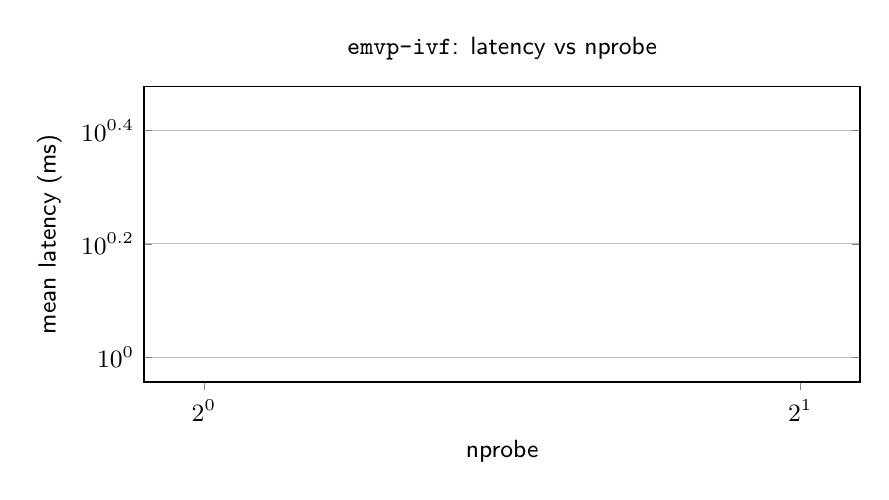
\begin{tikzpicture}
  \begin{axis}[
    xmode=log, log basis x=2, ymode=log,
    xlabel={nprobe},
    ylabel={mean latency (ms)},
    title={\texttt{emvp-ivf}: latency vs nprobe},
    legend columns=3,
  ]
    \foreach \slug/\dlabel in \canonicalSeries {%
      \IfFileExists{\datadir/01-latency-vs-nprobe-emvp-ivf-\slug.tsv}{%
        \edef\xtemp{%
          \noexpand\addplot+ table[x=nprobe, y=latency_ms]
            {\datadir/01-latency-vs-nprobe-emvp-ivf-\slug.tsv};%
          \noexpand\addlegendentry{\dlabel}%
        }\xtemp
      }{}%
    }
  \end{axis}
\end{tikzpicture}

  \caption{\texttt{emvp-ivf}: mean latency vs \texttt{nprobe}.
  Encrypted matrix-vector products are the dominant cost; cluster
  size scales the per-cluster compute linearly.}
\end{figure}

\begin{figure}[H]
  \centering
  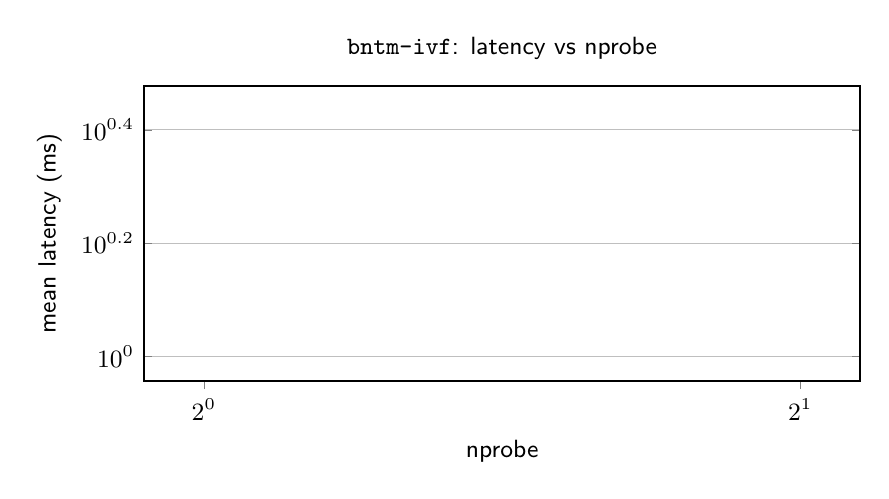
\begin{tikzpicture}
  \begin{axis}[
    xmode=log, log basis x=2, ymode=log,
    xlabel={nprobe},
    ylabel={mean latency (ms)},
    title={\texttt{bntm-ivf}: latency vs nprobe},
    legend columns=3,
  ]
    \foreach \slug/\dlabel in \canonicalSeries {%
      \IfFileExists{\datadir/01-latency-vs-nprobe-bntm-ivf-\slug.tsv}{%
        \edef\xtemp{%
          \noexpand\addplot+ table[x=nprobe, y=latency_ms]
            {\datadir/01-latency-vs-nprobe-bntm-ivf-\slug.tsv};%
          \noexpand\addlegendentry{\dlabel}%
        }\xtemp
      }{}%
    }
  \end{axis}
\end{tikzpicture}

  \caption{\texttt{bntm-ivf}: mean latency vs \texttt{nprobe}, with
  Protocol~2 verification on (the default).}
\end{figure}

\clearpage
\section{Per-machine latency at a canonical operating point}

Direct hardware ranking at the operating point each scheme converges
on (\texttt{nprobe=32} for IVF schemes, the lone config for flat
scorers). Easier to read than the log-log line plot when the
question is "which machine is fastest here?".

\IfFileExists{\datadir/02-bar-plaintext-nprobe-32.tikz}{%
\begin{figure}[H]
  \centering
  \inputplot{\datadir/02-bar-plaintext-nprobe-32.tikz}
  \caption{Per-machine mean latency for \texttt{plaintext} at
  \texttt{nprobe=32}. Bars sorted by latency.}
\end{figure}
}{}

\IfFileExists{\datadir/02-bar-sap-ivf-beta-0-0000-nprobe-32.tikz}{%
\begin{figure}[H]
  \centering
  \inputplot{\datadir/02-bar-sap-ivf-beta-0-0000-nprobe-32.tikz}
  \caption{Per-machine mean latency for \texttt{sap-ivf} at
  $\beta=0$, \texttt{nprobe=32}.}
\end{figure}
}{}

\IfFileExists{\datadir/02-bar-emvp-ivf-nprobe-32.tikz}{%
\begin{figure}[H]
  \centering
  \inputplot{\datadir/02-bar-emvp-ivf-nprobe-32.tikz}
  \caption{Per-machine mean latency for \texttt{emvp-ivf} at
  \texttt{nprobe=32}.}
\end{figure}
}{}

\IfFileExists{\datadir/02-bar-bntm-ivf-nprobe-32.tikz}{%
\begin{figure}[H]
  \centering
  \inputplot{\datadir/02-bar-bntm-ivf-nprobe-32.tikz}
  \caption{Per-machine mean latency for \texttt{bntm-ivf} at
  \texttt{nprobe=32}, verification on.}
\end{figure}
}{}

\IfFileExists{\datadir/02-bar-sap-beta-0-0000.tikz}{%
\begin{figure}[H]
  \centering
  \inputplot{\datadir/02-bar-sap-beta-0-0000.tikz}
  \caption{Per-machine mean latency for the flat \texttt{sap}
  scorer at $\beta=0$.}
\end{figure}
}{}

\IfFileExists{\datadir/02-bar-emvp-emvp.tikz}{%
\begin{figure}[H]
  \centering
  \inputplot{\datadir/02-bar-emvp-emvp.tikz}
  \caption{Per-machine mean latency for the flat \texttt{emvp}
  scorer.}
\end{figure}
}{}

\IfFileExists{\datadir/02-bar-bntm-bntm.tikz}{%
\begin{figure}[H]
  \centering
  \inputplot{\datadir/02-bar-bntm-bntm.tikz}
  \caption{Per-machine mean latency for the flat \texttt{bntm}
  scorer.}
\end{figure}
}{}

\clearpage
\section{Parallel scaling}

For machines with a recorded thread sweep at the canonical operating
point (\texttt{nprobe=32}; Plan~13's \texttt{eval-scaling} sweep is
the natural source). Lines on a single (machine, device, cgroup)
tuple expose the diminishing-returns curve of additional cores.

\begin{figure}[H]
  \centering
  \input{figures/03-parallel-scaling-plaintext}
  \caption{\texttt{plaintext} @ \texttt{nprobe=32}: mean latency vs
  realised rayon thread count.}
\end{figure}

\begin{figure}[H]
  \centering
  \input{figures/03-parallel-scaling-sap-ivf}
  \caption{\texttt{sap-ivf} @ $\beta=0$, \texttt{nprobe=32}: mean
  latency vs realised threads.}
\end{figure}

\begin{figure}[H]
  \centering
  \input{figures/03-parallel-scaling-emvp-ivf}
  \caption{\texttt{emvp-ivf} @ \texttt{nprobe=32}: mean latency vs
  realised threads.}
\end{figure}

\begin{figure}[H]
  \centering
  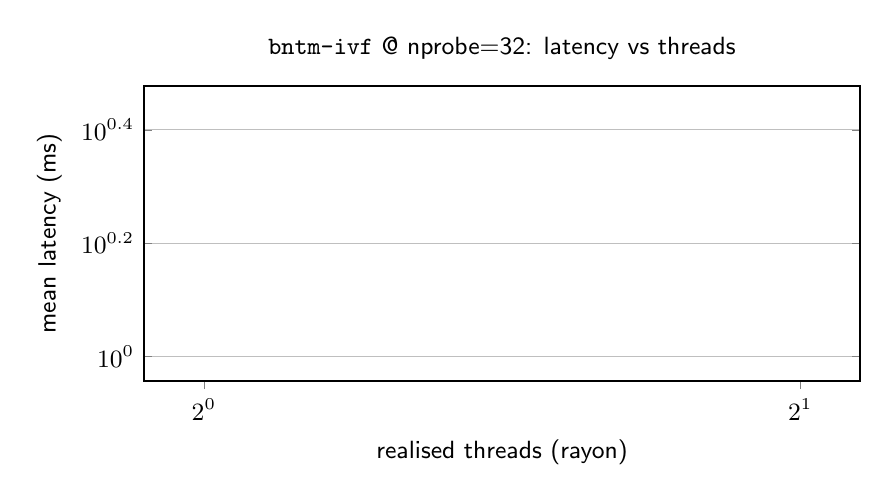
\begin{tikzpicture}
  \begin{axis}[
    xmode=log, log basis x=2, ymode=log,
    xlabel={realised threads (rayon)},
    ylabel={mean latency (ms)},
    title={\texttt{bntm-ivf} @ nprobe=32: latency vs threads},
    legend style={
      at={(0.02,0.02)}, anchor=south west,
      draw=none, fill=white, fill opacity=0.85, text opacity=1,
      font=\sffamily\footnotesize,
    },
    legend columns=1,
  ]
    \foreach \slug/\dlabel in \canonicalSeries {%
      \IfFileExists{\datadir/03-parallel-scaling-bntm-ivf-nprobe-32-\slug.tsv}{%
        \edef\xtemp{%
          \noexpand\addplot+ table[x=threads, y=latency_ms]
            {\datadir/03-parallel-scaling-bntm-ivf-nprobe-32-\slug.tsv};%
          \noexpand\addlegendentry{\dlabel}%
        }\xtemp
      }{}%
    }
  \end{axis}
\end{tikzpicture}

  \caption{\texttt{bntm-ivf} @ \texttt{nprobe=32}, verification on:
  mean latency vs realised threads.}
\end{figure}

\end{document}
